\documentclass[10pt]{beamer}
\usepackage[T1]{fontenc}
\usepackage[utf8]{inputenc}

\graphicspath{{}{figures/}}

\usetheme[progressbar=frametitle]{metropolis}
\usepackage{appendixnumberbeamer}

\usepackage{booktabs}
\usepackage[scale=2]{ccicons}

\usepackage{pgfplots}
\pgfplotsset{compat=1.12}
\usepgfplotslibrary{dateplot}

\usetikzlibrary{calc,fit,patterns}
\usepackage[absolute,overlay]{textpos}

\usepackage{xspace}
\newcommand{\themename}{\textbf{\textsc{metropolis}}\xspace}

\usepackage{xcolor}
\usepackage{listings}
\lstset{columns=fullflexible}
\lstdefinelanguage{EOL}{
morekeywords={delete,import,for,while,in,and,or,self,operation,return,def,var,throw,if,new,else,transaction,abort,
break,breakAll,continue,assert,assertError,not, switch, case, default},
sensitive=true,
morecomment=[l]{//},
morecomment=[l]{--},
morecomment=[s]{/*}{*/},
morecomment=[s]{-*}{*-},
morestring=[b]",
morestring=[b]',
showstringspaces=false
}

\lstnewenvironment{java}{\lstset{language=Java,
		frame=tb,
        tabsize=3,
        morekeywords={implies, in, result},
        basicstyle=\footnotesize,
        keywordstyle=\bfseries,
        ndkeywordstyle=\bfseries,
        commentstyle=\itshape,
		morecomment=[l]{--},
        stringstyle=\ttfamily,
		showspaces=false,
        flexiblecolumns,
        literate={->}{$\to$}{2} {--}{-$\,$-}{2} {<=}{$\le$}{2} {>=}{$\ge$}{2} {<>}{$<\,>$}{3},
        sensitive, extendedchars, texcl}}{}

\lstnewenvironment{ocl}{\lstset{language=[decorative]OCL,
	frame=tb,
	tabsize=3,
	morekeywords={implies,result,flatten,body,init,OrderedSet,Tuple,TupleType,def,attr,oclIsUndefined,oclIsInvalid,OclState,let,in},
	basicstyle=\footnotesize,
	keywordstyle=\bfseries,
	ndkeywordstyle=\bfseries,
	commentstyle=\itshape,
	stringstyle=\ttfamily,
	showspaces=false,
	flexiblecolumns,
	literate={->}{$\to$}{2} {--}{-$\,$-}{2} {<=}{$\le$}{2} {>=}{$\ge$}{2} {<>}{$<\,>$}{3},
	sensitive, extendedchars, texcl}}{}


\lstdefinelanguage{gremlin}{
morekeywords={as,def,fill,filter,groupCount,has,idx,inE,inV,is,label,length,match,outE,outV,v,values},
sensitive=true,
morecomment=[l]{//}
}

% "page cs" coordinate system
% From http://tex.stackexchange.com/questions/89588/
%
% Defining a new coordinate system for the page:
%
% --------------------------
% |(-1,1)    (0,1)    (1,1)|
% |                        |
% |(-1,0)    (0,0)    (1,0)|
% |                        |
% |(-1,-1)   (0,-1)  (1,-1)|
% --------------------------
\makeatletter
\def\parsecomma#1,#2\endparsecomma{\def\page@x{#1}\def\page@y{#2}}
\tikzdeclarecoordinatesystem{page}{
    \parsecomma#1\endparsecomma
    \pgfpointanchor{current page}{north east}
    % Save the upper right corner
    \pgf@xc=\pgf@x%
    \pgf@yc=\pgf@y%
    % save the lower left corner
    \pgfpointanchor{current page}{south west}
    \pgf@xb=\pgf@x%
    \pgf@yb=\pgf@y%
    % Transform to the correct placement
    \pgfmathparse{(\pgf@xc-\pgf@xb)/2.*\page@x+(\pgf@xc+\pgf@xb)/2.}
    \expandafter\pgf@x\expandafter=\pgfmathresult pt
    \pgfmathparse{(\pgf@yc-\pgf@yb)/2.*\page@y+(\pgf@yc+\pgf@yb)/2.}
    \expandafter\pgf@y\expandafter=\pgfmathresult pt
}
\makeatother
% Draws a grid for easier referencing of page cs values
\newcommand{\printtikzpagegrid}{
  \tiny
  \begin{tikzpicture}[overlay,remember picture,every node/.style={inner sep=.1em,draw=black!20,fill=white}]
    \foreach \x in {0,...,9} {
      \foreach \y in {0,...,9} {
        \node at (page cs:0.\x,0.\y) {};
        \node at (page cs:0.\x,-0.\y) {};
        \node at (page cs:-0.\x,0.\y) {};
        \node at (page cs:-0.\x,-0.\y) {};
      }
    }
    \node at (page cs:0,0) {0,0};
    \node at (page cs:0.5,0.5) {.5,.5};
    \node at (page cs:0.5,-0.5) {.5,-.5};
    \node at (page cs:-0.5,0.5) {-.5,.5};
    \node at (page cs:-0.5,-0.5) {-.5,-.5};
    \node at (page cs:1,1) {1,1};
    \node at (page cs:1,-1) {1,-1};
    \node at (page cs:-1,1) {-1,1};
    \node at (page cs:-1,-1) {-1,-1};
  \end{tikzpicture}
  \normalsize
}

\title{Taming Large Models\\with Hawk and NeoEMF}
%\subtitle{A modern beamer theme}
\date{MoDELS'2018, 14--19 October 2018}
\author{A. García-Domínguez, D. S. Kolovos, K. Barmpis, G. Daniel, G. Sunyé}
%\institute{Center for modern beamer themes}
% \titlegraphic{\hfill\includegraphics[height=1.5cm]{logo.pdf}}

\begin{document}

\maketitle

\begin{frame}{Table of contents}
  \setbeamertemplate{section in toc}[sections numbered]
  \tableofcontents[hideallsubsections]
\end{frame}

\section{Introduction}

\begin{frame}{Who are we? --- Hawk team}
\centering

\begin{columns}
\column{.3\textwidth}
\centering
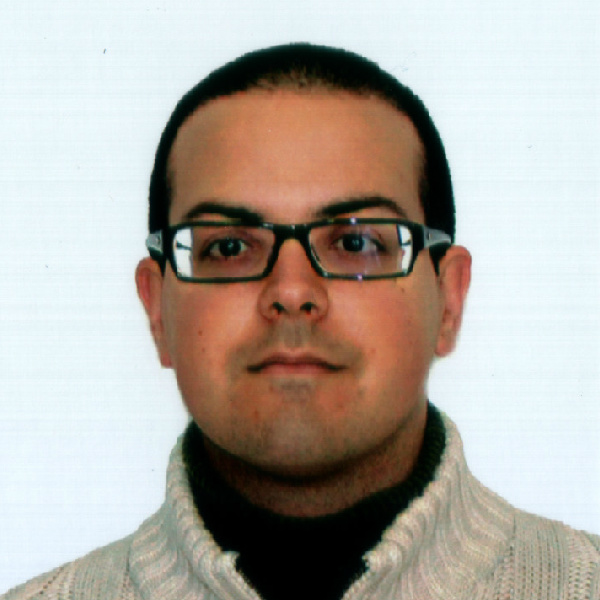
\includegraphics[height=.25\textheight]{biopic-01-antonio}
\column{.7\textwidth}
\begin{block}{Antonio (Lecturer, Aston University)}
\begin{itemize}
\item Hawk project lead
\item Eclipse Epsilon committer
\end{itemize}
\end{block}
\end{columns}

\begin{columns}
\column{.3\textwidth}
\centering
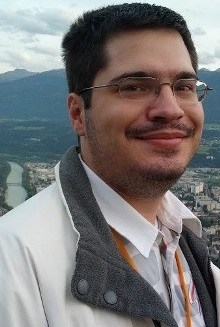
\includegraphics[height=.25\textheight,clip,trim={0 3cm 0 0}]{biopic-02-konstantinos}
\column{.7\textwidth}
\begin{block}{Konstantinos (Research Associate, U.\ of York)}
\begin{itemize}
\item Hawk initiator (core developer)
\item Created most core components
\end{itemize}
\end{block}
\end{columns}

\begin{columns}
\column{.3\textwidth}
\centering
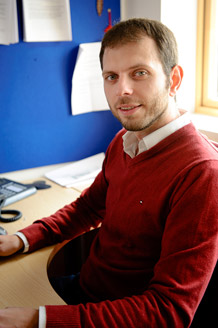
\includegraphics[height=.25\textheight,clip,trim={0 4cm 0 0}]{biopic-03-dimitris}
\column{.7\textwidth}
\centering
\begin{block}{Dimitris (Professor, University of York)}
\begin{itemize}
\item Hawk initiator (MONDO WP lead)
\item Eclipse Epsilon project lead
\end{itemize}
\end{block}
\end{columns}

\end{frame}

\begin{frame}{Who are we? --- NeoEMF team}

\begin{columns}
\column{.3\textwidth}
\centering
%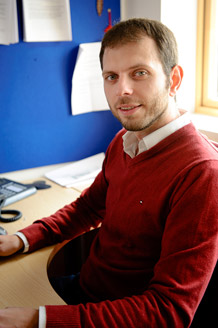
\includegraphics[height=.25\textheight,clip,trim={0 4cm 0 0}]{biopic-03-dimitris}
\column{.7\textwidth}
\centering
\begin{block}{Gwendal (Post-doc, SOM Research Lab)}
\begin{itemize}
\item NeoEMF core developer
\item Mogwaï project lead
\end{itemize}
\end{block}
\end{columns}

\begin{columns}
\column{.3\textwidth}
\centering
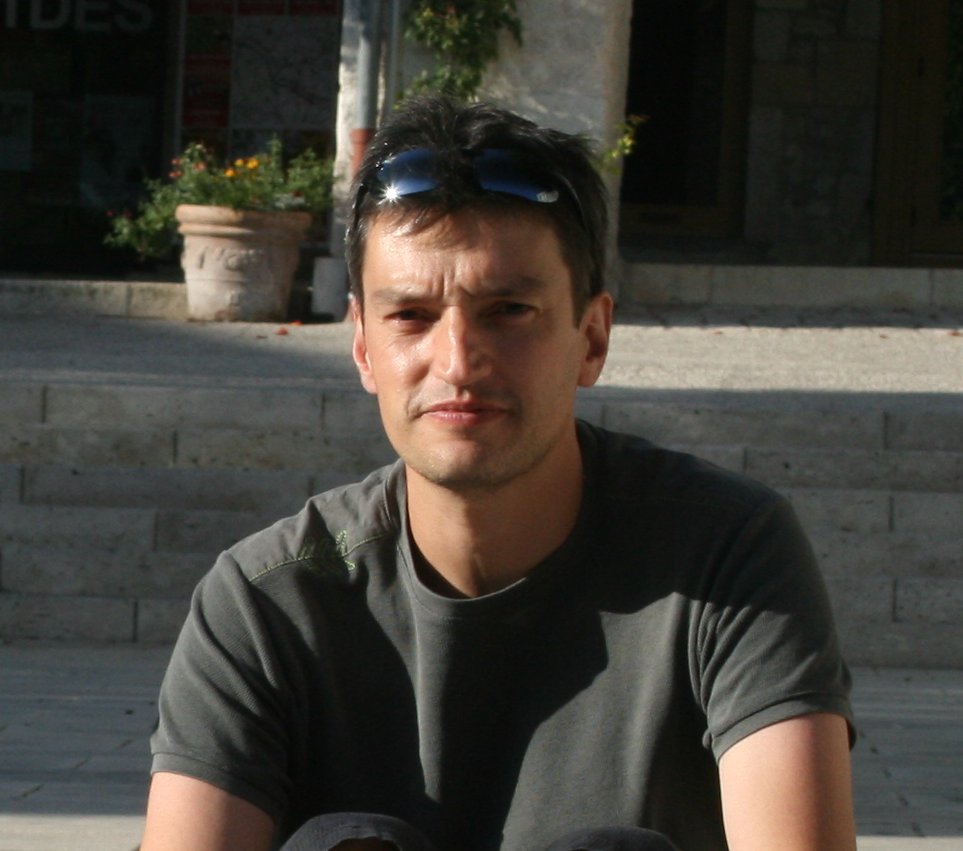
\includegraphics[height=.25\textheight,clip,trim={0 3cm 0 0}]{biopic-04-gerson}
\column{.7\textwidth}
\begin{block}{Gerson (Associate Professor, U.\ of Nantes)}
\begin{itemize}
\item NeoEMF initiator
\item AtlanMod project lead
\end{itemize}
\end{block}
\end{columns}

\end{frame}

\begin{frame}{Motivation: monolithic XMI models do not scale}
\centering

\begin{quote}
``[Lack of] Scalability is what is holding back a number of potential adopters''~\cite{Barmpis2013}
\end{quote}

\begin{quote}
``One can easily observe that scalability is the most critical of today's (and tomorrow's) challenges''~\cite{Mougenot2009}
\end{quote}

\begin{table}
\begin{tabular}{rrrr}
\toprule
Model & XMI (MB) & Avg.\ memory (MB) & Max memory (MB) \\
\midrule
%set0 & 8.75 & 22 & 49 \\
set1 & 26.59 & 53 & 135 \\
set2 & 270.12 & 437 & 840 \\
set3 & 597.67 & 849 & 1798 \\
set4 & 645.53 & 949 & 1910 \\
\bottomrule
\end{tabular}

\caption{Querying GraBaTs'09 Java models to find singletons}
\end{table}

\end{frame}

\begin{frame}{What to do?}

\begin{block}{Option 1: break up into fragments}
  \begin{itemize}
  \item Code is broken up into modules --- do the same with models
  \item Fragmented file-based models play well with traditional VCS
  \item Global queries may still require loading all fragments!
  \item \textbf{\alert{Hawk}} is our solution: indexes the fragments into a NoSQL database, queries the database instead of the fragments
  \end{itemize}
\end{block}

\begin{block}{Option 2: stop using files}
  \begin{itemize}
  \item Obviously not new: CDO has been doing it for years
  \item However, relational DBs are not the only option
  \item \textbf{\alert{NeoEMF}} can replace traditional XMI persistence with
    NoSQL approaches: graph databases, key-value stores...
  \end{itemize}
\end{block}

\end{frame}

\begin{frame}{Basic concepts about NoSQL}

\begin{block}{NoSQL = not only SQL}
  \begin{itemize}
  \item Generally, non-relational databases
  \item Some improve availability/performance by relaxing ACID
  \item Some are focused on specific analyses (e.g. social graphs)
  \end{itemize}
\end{block}

\begin{block}{Common types}
\begin{itemize}
\item \textbf{Key-value stores} implement an associative array to quickly fetch
  records given a tuple-based identifier (e.g. RocksDB, Redis).

\item \textbf{Document stores} keep collections of heterogeneous docs
  retrievable by key, supporting hierarchies + querying by field (e.g. MongoDB).

\item \textbf{Graph databases} store nodes, edges and their fields (e.g. Neo4j,
  OrientDB). Many support indexing and have query languages.

\item \textbf{Tuple stores} store subject-predicate-object triples (e.g. RDF4J,
  Jena). Very often used in Semantic Web approaches.
\end{itemize}
\end{block}

\end{frame}

\begin{frame}{Some considerations before we start}

  \begin{block}{NoSQL = purpose-specific databases}
    \begin{itemize}
    \item Can provide better capabilities than RDBMS, but require careful choice
      + benchmarking + tuning --- luckily, we did this for you :-)
    \item Technology/release/API all impact performance:
      \begin{itemize}
      \item Hawk Neo4j backend still in v2.0.5: later v2.x \emph{were slower},
        as Neo4j optimized for different requirements
      \item Hawk OrientDB v2.2.30 backend avoids \emph{slower} official OrientDB
        graph API, and uses the core document API instead
      \end{itemize}
    \end{itemize}
  \end{block}

  \begin{block}{Consider your requirements}
    \begin{itemize}
    \item Do you need faster queries?
    \item Do you need faster loading/saving? If so:
      \begin{itemize}
      \item Can you break up your files into fragments?
      \item Can you save to disk only the fragments that changed?
      \end{itemize}
    \end{itemize}

    We will revisit these during the wrap-up.
  \end{block}

\end{frame}

\pgfset{/metropolis/inner/sectionpage/.cd, none}

\section{Hawk}

\section{NeoEMF}

\section{Mogwa\"i}

\section{Wrap-up}

\appendix

\begin{frame}[standout]
  Done with intro --- let's start with Hawk!
\end{frame}

\begin{frame}{References}

  \bibliography{../bibliography}
  \bibliographystyle{alpha}

\end{frame}

\end{document}
